% !TeX encoding = UTF-8
% !TEX TS-program = xelatex


\documentclass{beamer}
\usepackage{ctex}
\renewcommand{\today}{2021~年~5~月~25~日}
%\CTEXoptions[today=old]

\usetheme{CambridgeUS}
\pgfdeclareimage[width=\paperwidth,height=\paperheight]{bg}{figures/seu_background}
\setbeamertemplate{background}{\pgfuseimage{bg}}
\setbeamertemplate{blocks}[rounded][shadow=true]
%\addtobeamertemplate{block begin}{}{\justifying}
% gets rid of navigation symbols
%\setbeamertemplate{navigation symbols}{}

% add figures numbering
%\setbeamertemplate{caption}[numbered]


%\usepackage{cmbright} % computer modern font sans serif
\usepackage{graphicx} % Allows including images
\usepackage{booktabs} % Allows the use of \toprule, \midrule and \bottomrule in tables
\usepackage{appendixnumberbeamer} % Number for appendix numbers
\usepackage{ragged2e}
\usepackage{amsmath}
\usepackage{amssymb}
\usepackage{amsfonts}
\usepackage{mathrsfs}
\usepackage{subfigure}
\graphicspath{{./image/}}
\usepackage{hyperref}
\hypersetup{
%bookmarks=true,                    % show bookmarks bar?
unicode=false,                      % non-Latin characters in Acrobat’s bookmarks
pdftoolbar=true,                    % show Acrobat’s toolbar?
pdfmenubar=true,                    % show Acrobat’s menu?
pdffitwindow=false,                 % window fit to page when opened
pdfstartview={FitH},                % fits the width of the page to the window
%pdftitle={My title},               % title
%pdfauthor={Author},                % author
%pdfsubject={Subject},              % subject of the document
%pdfcreator={Creator},              % creator of the document
%pdfproducer={Producer},            % producer of the document
%pdfkeywords={keyword1} {key2},     % list of keywords
%pdfnewwindow=true,                 % links in new window
colorlinks=true,                    % false: boxed links; true: colored links
linkcolor=black,                    % color of internal links (change box color with linkbordercolor)
citecolor=green,                    % color of links to bibliography
filecolor=magenta,                  % color of file links
urlcolor=red                    % color of external links
}


% gets rid of bottom navigation bars
%\setbeamertemplate{footline}[page number]{}
%\setbeamertemplate{headline}{}
%\setbeamerfont{frametitle}{family=\bfseries}
%\setbeamerfont{myTOC}{series=\bfseries,size=\normalfont}
%\usebeamerfont{myTOC}\tableofcontents[current]}}


\beamertemplateballitem
\AtBeginSection[]
{
\begin{frame}<beamer>
\frametitle{\textbf{目录}}
\textbf{\tableofcontents[currentsection]}
\end{frame}
}



\title[Sending out an SMS]{Sending out an SMS: Characterizing the Security of the SMS Ecosystem with Public Gateways}
\subtitle{利用公共网关的SMS生态系统的安全性描述}

\author[名字缩写]{名字\\
xxx@seu.edu.cn}

\institute[SEU]
{信息科学与工程学院 \\
东南大学  \\ \vspace{.3cm}
\centering 
\includegraphics[width=0.13\linewidth]{figures/seu-color-logo}  
}

\date{\today}

	

\begin{document}
%------------------------------------------------
\begin{frame}
\titlepage
\end{frame}

\section*{目录}

\begin{frame}
\frametitle{\textbf{目录}}
\textbf{\tableofcontents}
\end{frame}	


\section{引言}

\begin{frame}
\frametitle{\textbf{引言}}
\begin{block}{\textbf{研究背景}}
\begin{itemize}
    \item 短信息(SMS)成为现代通讯的重要组成部分
    \item 很多组织或网站使用短信息作为身份验证的辅助通道
    \item 现代短消息的发送,在抵达终端之前不接触蜂窝网络
\end{itemize}
\end{block}

\begin{block}{\textbf{主要工作}}
\begin{itemize}
    \item 对SMS数据进行迄今为止最大的挖掘分析
    \item 评估良性短消息服务的安全态势
    \item 刻画通过SMS网关进行的恶意行为
\end{itemize}
\end{block}
\end{frame}

\section[系统]{现代SMS生态系统}

\begin{frame}
\frametitle{\textbf{短消息服务中心(SMSC)}}
\begin{figure}[!t]
\centering
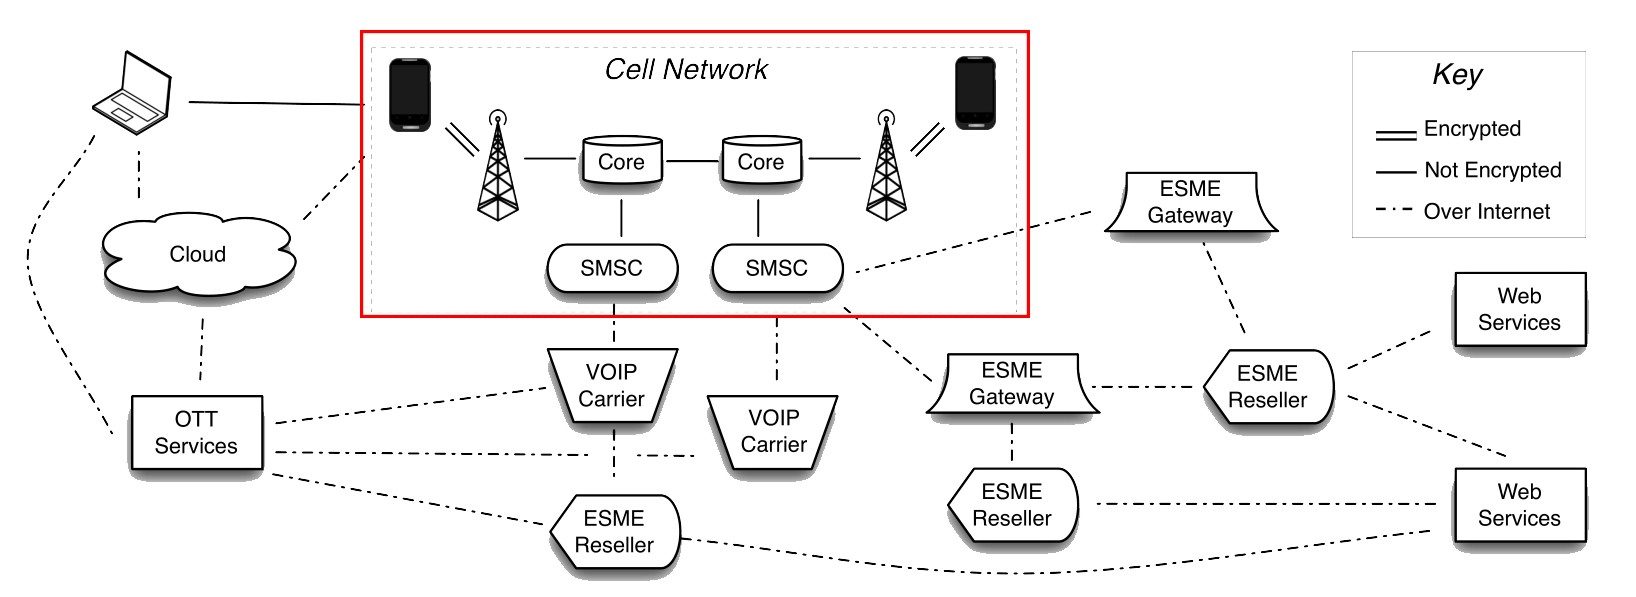
\includegraphics[width=4in]{beamer/figure1.png}
\caption{短消息服务中心}
\label{figure1_SMSC}
\end{figure}
\textbf{短消息服务中心}通过运营商网络路由消息,是SMS系统的核心。\\
SMSC接受文本消息,并将消息转发到蜂窝网络中的移动用户。
\end{frame}

\begin{frame}
\frametitle{\textbf{外部短消息实体(ESME)}}
\begin{figure}[!t]
\centering
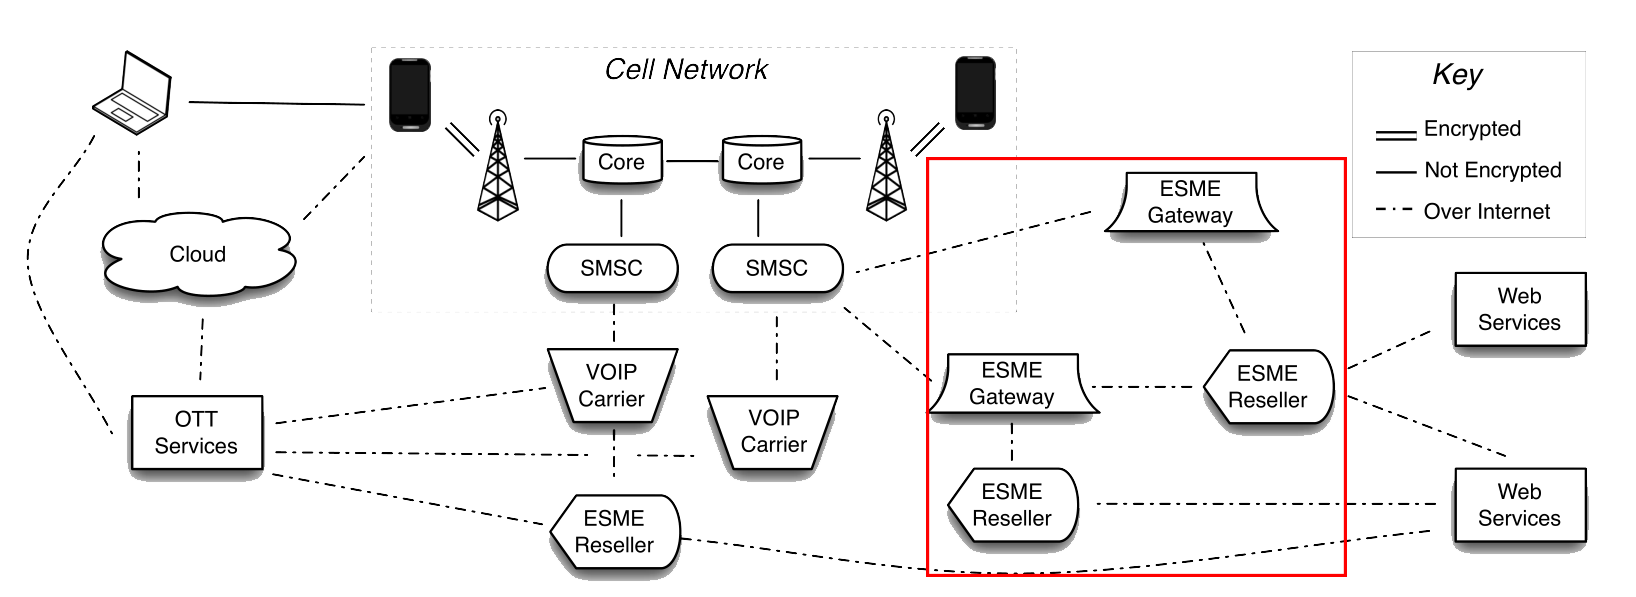
\includegraphics[width=4in]{beamer/figure2.png}
\caption{外部短消息实体}
\label{figure2_ESME}
\end{figure}
\textbf{外部短消息实体}为外部组织提供针对运营商网络的短消息接入服务。\\
ESME可以用于紧急通报、慈善捐款、或接受一次性验证码等功能。
\end{frame}

\begin{frame}
\frametitle{\textbf{OTT服务}}
\begin{figure}[!t]
\centering
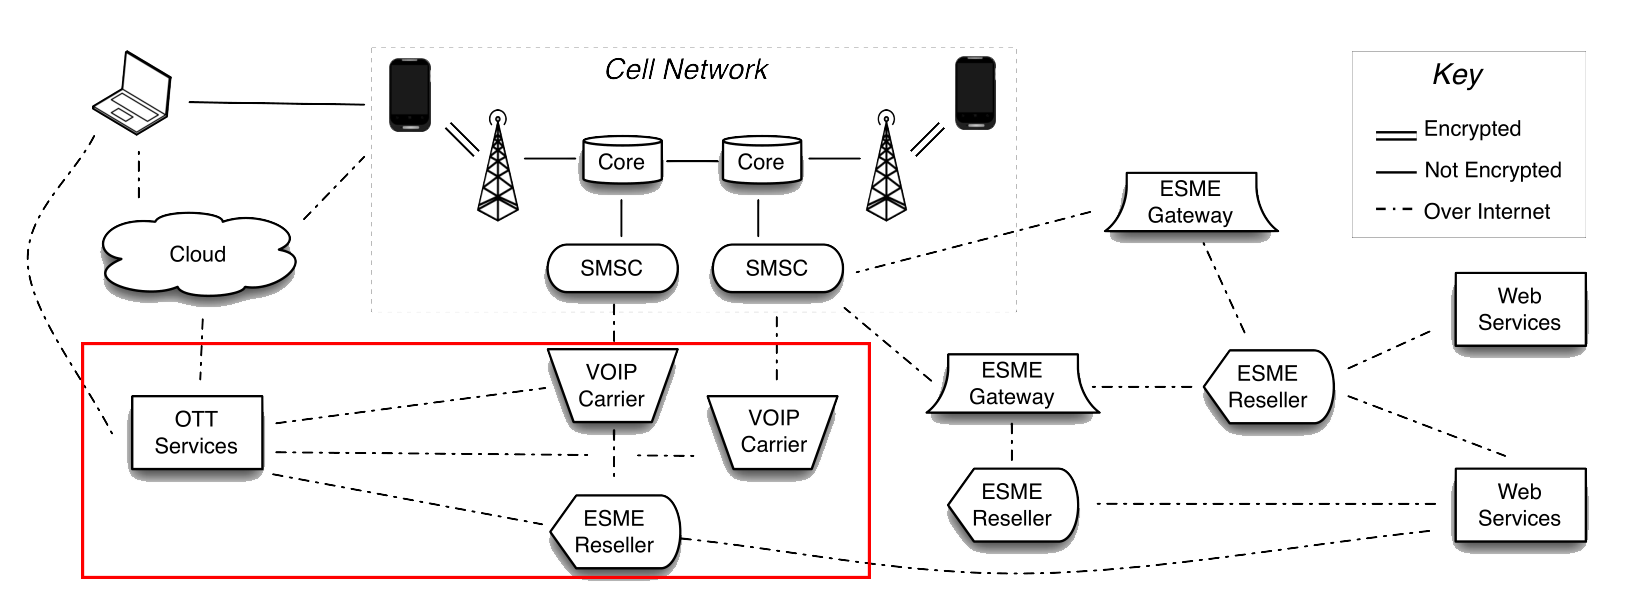
\includegraphics[width=4in]{beamer/figure3.png}
\caption{OTT服务}
\label{figure3_OTT}
\end{figure}
\textbf{OTT服务}支持在数据网络上提供短信和语音等第三方服务。\\
OTT可以使用云服务来存储和同步SMS到用户的其他设备。
\end{frame}



\section[方法]{研究方法与数据集特征}


\begin{frame}
\frametitle{\textbf{爬取公共短消息网关}}
% ----------------分栏的结构开始---------------- %
% 该结构中使用block分开两个内容区
% 可根据需要进行图文混排?我还没试过,我想应该可以
\begin{columns}
\column{.5\textwidth}
\footnotesize
\begin{itemize}
    \item 使用Scrapy框架爬取公共网关
    \item 收集8个公共短信网关在14个月的数据
    \item 共抓取386,327条数据
\end{itemize}

\column{.5\textwidth}
\begin{table}
\caption{公共网关及抓取的信息数}
\label{table1:gateways}
\centering
\footnotesize
\begin{tabular}{|c|c|}
\hline
\textbf{Site}           & \textbf{Messages}\\
\hline
receivesmsonline.net    &81313\\
\hline
receive-sms-online.info &69389\\
\hline
receive-sms-now.com     &63797\\
\hline
    hs3x.com               &55499\\
\hline
receivesmsonline.com    &44640\\
\hline
receivefreesms.com      &37485\\
\hline
receive-sms-online.com  &27094\\
\hline
    e-receivesms.com       &7107\\
\hline
\end{tabular}
\end{table}
\end{columns}

\end{frame}

\begin{frame}
\frametitle{\textbf{消息聚类分析}}
\begin{block}{\textbf{基本思路}}
\begin{itemize}
    \item 使用编辑距离矩阵将类似的消息归于一张连通图中。
    \item 使用固定值替换感兴趣的消息,如代码、email地址。
    \item 查找归一化距离小于阈值的消息,并确定聚类边界。
\end{itemize}
\end{block}

\begin{block}{\textbf{实现步骤}}
\begin{enumerate}
    \item 加载所有消息。
    \item 用固定的字符串替换数字、电子邮件和URL以预处理消息。
    \item 将预处理后的信息按字母排序。
    \item 通过使用编辑距离阈值(0.9)来确定聚类边界。
    \item 手动标记各个聚类,以确定服务提供者、消息类别等。
\end{enumerate}
\end{block}
\end{frame}

\begin{frame}
\frametitle{\textbf{消息分类结果}}
\begin{itemize}
\item \textbf{账户创建确认信息}:向来自服务提供者的用户提供了一个代码,该服务提供者需要在新帐户创建期间进行SMS验证。
\item \textbf{活动确认信息}:向来自服务提供者的用户提供了请求授权进行活动的代码(例如,付款确认)。
\item \textbf{一次性密码}:包含用户登录的代码的短信息。
\item \textbf{用于绑定不同设备的一次性口令}:将消息发送给用户,以绑定一个新的电话号码或启用相应的移动应用程序。
\item \textbf{重置密码口令}:包含密码重置密码的短信息。
\item \textbf{其他}:其他未被指定为某种特定功能的消息。
\end{itemize}
\end{frame}

\begin{frame}
\frametitle{\textbf{消息分类结果}}
\begin{columns}
\column{.5\textwidth}
\footnotesize
\begin{itemize}
    \item 账户创建和移动设备绑定占比最大,占51.6\%
    \item 一次性密码信息占7.6\%
    \item 密码重置消息占1.3\%
    \item 包含“测试”关键词的消息占0.8\%
\end{itemize}

\column{.5\textwidth}
\begin{figure}[!t]
    \centering
    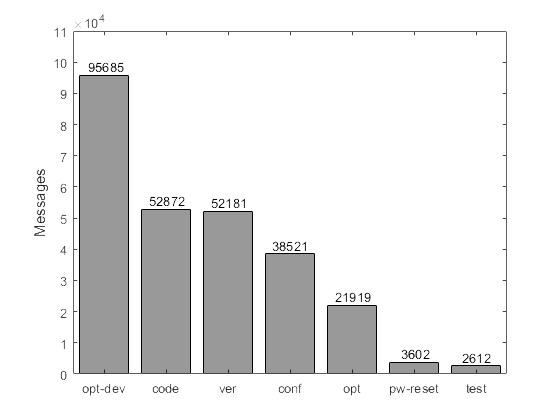
\includegraphics[width=1.1\textwidth]{beamer/figure4.png}
    \caption{消息的聚类}
    \label{figure3_OTT}
\end{figure}
\end{columns}
\end{frame}



\section[分析]{SMS使用情况分析}


\begin{frame}
\frametitle{\textbf{使用SMS作为安全信道}}
\begin{block}{\textbf{PII和其他敏感信息}}
\begin{itemize}
    \item 财务信息
    \item 用户名和密码
    \item 重置密码口令
    \item 其他个人识别信息(PII)
    \item 敏感程序的SMS活动
\end{itemize}
\end{block}
\end{frame}

\begin{frame}
\frametitle{\textbf{使用SMS作为安全信道}}
\begin{block}{\textbf{SMS编码熵}}
使用 $\chi$方检验测试每组编码的熵。$\chi$方检验是一个零假设的显著性检验,用于测试SMS服务的编码是否是从低位到高位均匀分布的。若p值小于0.01,则表明观测值和理想均匀分布之间存在统计学上的显著差异。
检验结果表明,65\%的SMS服务的编码熵较低,容易被预测和攻击。
\end{block}
\begin{columns}

\column{.26\textwidth}
\begin{figure}
    \centering
    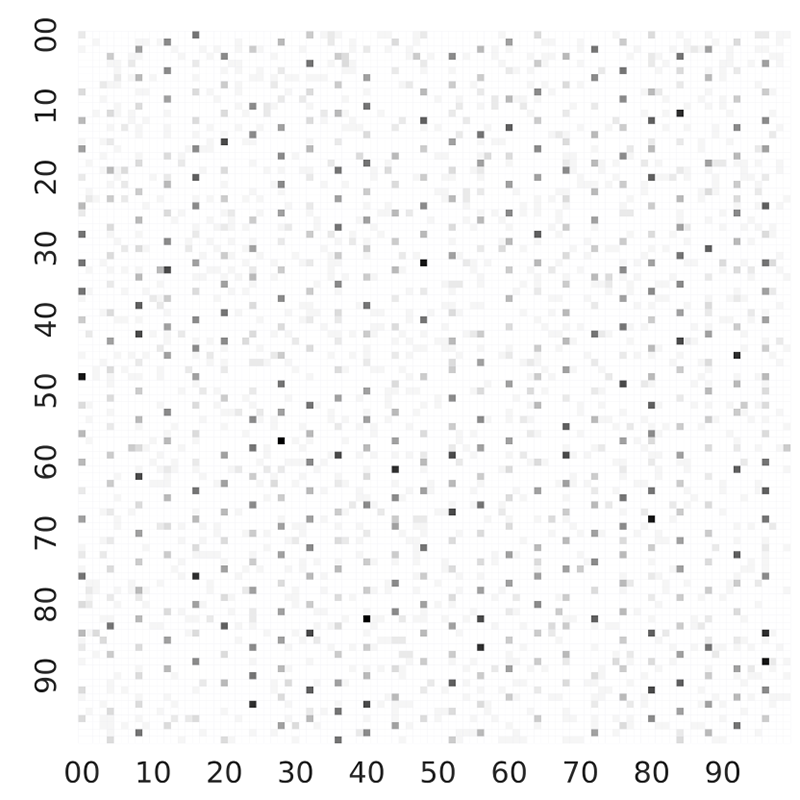
\includegraphics[width=1.1\textwidth]{beamer/figure6.png}
    \caption{WeChat}
    \label{figure6_WeChat}
\end{figure}

\column{.26\textwidth}
\begin{figure}
    \centering
    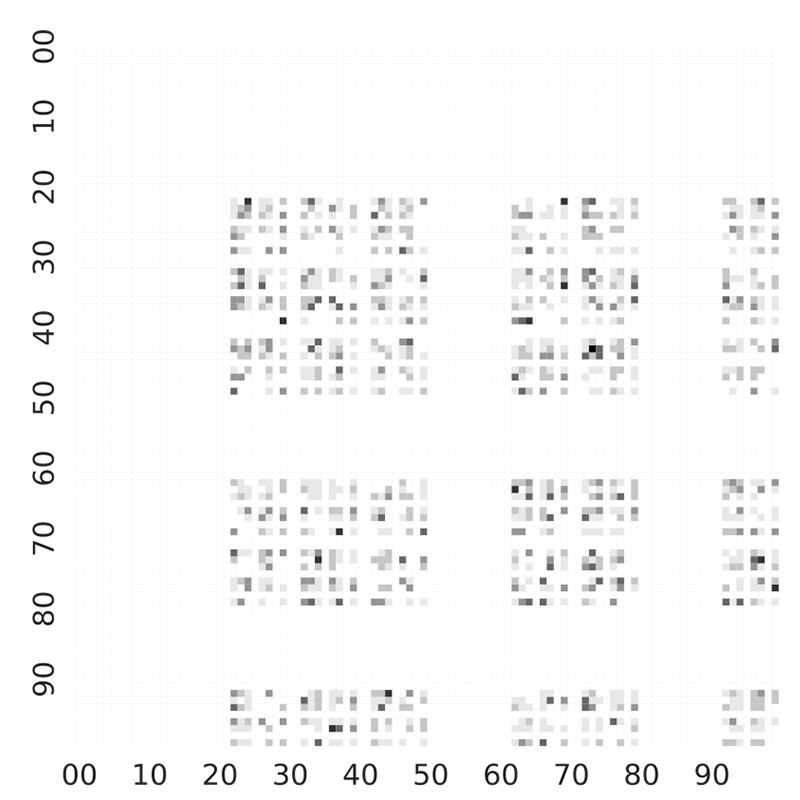
\includegraphics[width=1.1\textwidth]{beamer/figure7.png}
    \caption{Talk2}
    \label{figure3_Talk2}
\end{figure}

\column{.26\textwidth}
\begin{figure}
    \centering
    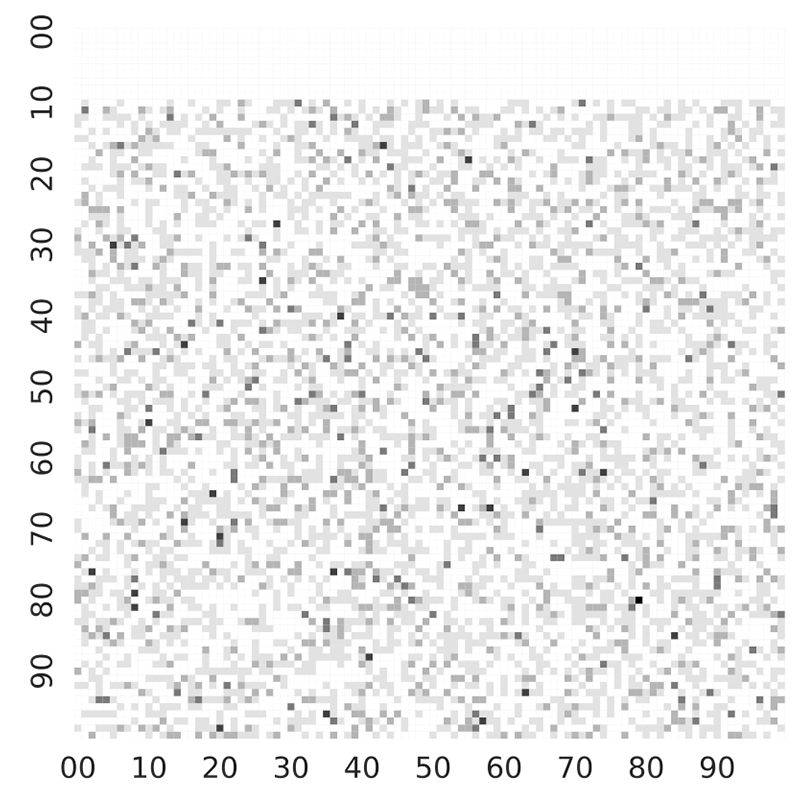
\includegraphics[width=1.1\textwidth]{beamer/figure8.png}
    \caption{Google}
    \label{figure3_Google}
\end{figure}

\end{columns}

\end{frame}

\begin{frame}
\frametitle{\textbf{SMS的恶意应用}}
\begin{block}{\textbf{公共网关检测到的恶意信息}}
\begin{itemize}
\item \textbf{泄露用户位置信息}:短URL可以用于确定消息的源和目的地,即会泄漏用户的位置信息。
\item \textbf{垃圾邮件宣传广告}:在公共网关服务中比例较低,约为1.0\%。
\item \textbf{网络钓鱼活动}:试图欺骗用户,使其相信自己正与合法网站通信。
\end{itemize}
\end{block}

\begin{columns}

\column{.26\textwidth}
\begin{figure}
    \centering
    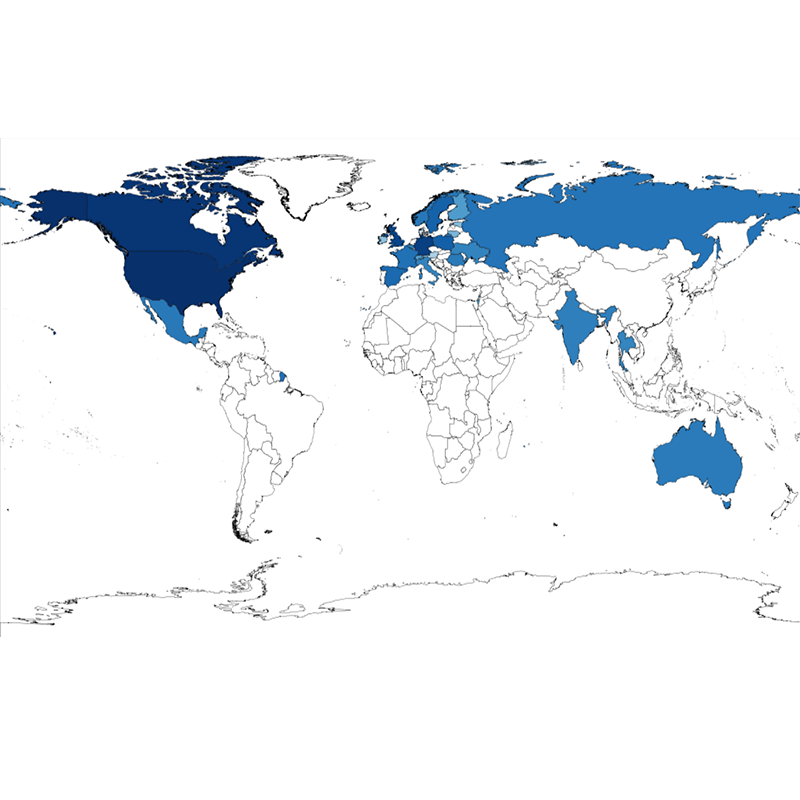
\includegraphics[width=1.1\textwidth]{beamer/figure9.png}
    \caption{SMS地址分布}
    \label{figure9_WeChat}
\end{figure}

\column{.26\textwidth}
\begin{figure}
    \centering
    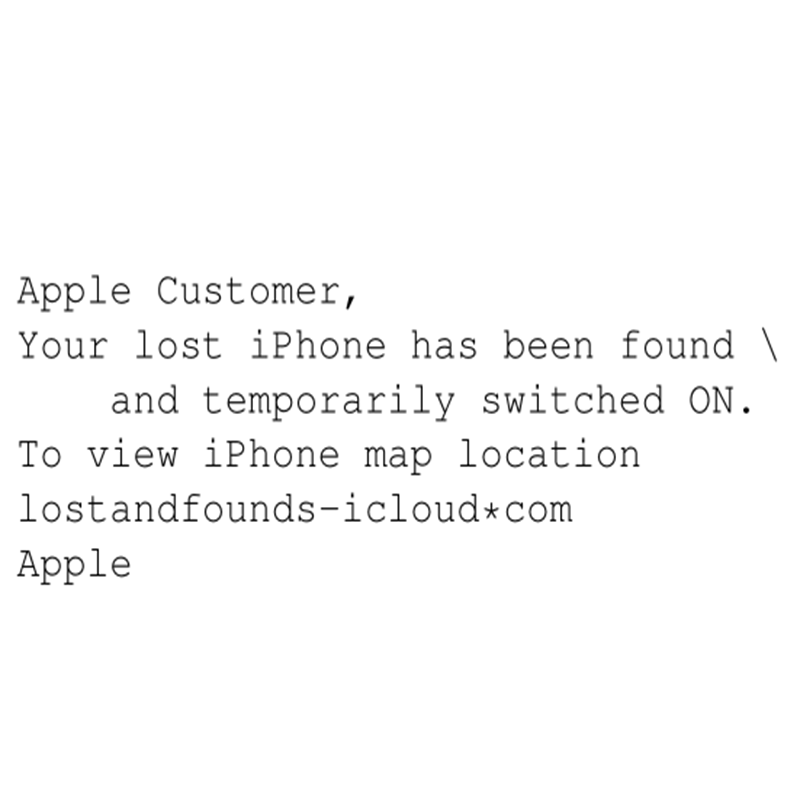
\includegraphics[width=1.1\textwidth]{beamer/figure10.png}
    \caption{钓鱼短信实例}
    \label{figure10_Talk2}
\end{figure}

\column{.26\textwidth}
\begin{figure}
    \centering
    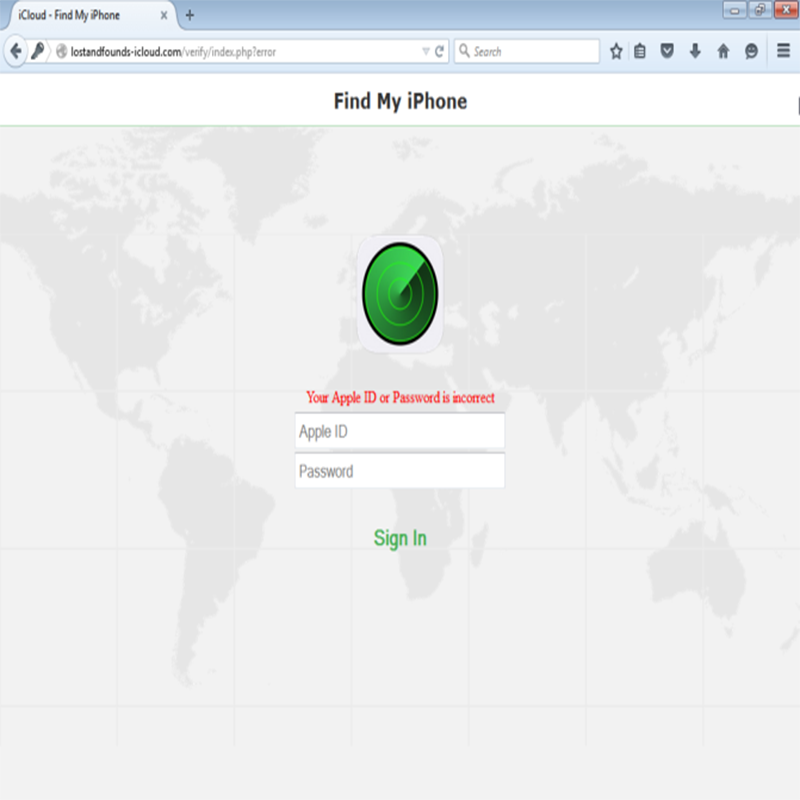
\includegraphics[width=1.1\textwidth]{beamer/figure11.png}
    \caption{钓鱼网站}
    \label{figure11_Talk2}
\end{figure}

\end{columns}

\end{frame}

\section[结论]{结论}


\begin{frame}
\frametitle{\textbf{结论}}

\begin{itemize}
\item SMS生态系统在智能手机时代出现了新的发展,加入了更多新的设备和参与者。
\item 公共网关为用户提供了基于SMS的各种安全解决方案。
\item 根据该研究,将SMS作为安全信道传递敏感信息存在一定的危险性。一些一次性的消息传递机制亟待改进。
\item 至于短信滥用,公共网关可以用于规避一些安全性较差的认证机制,或进行PVA欺诈行为。
\end{itemize}
\end{frame}



\section*{}
\begin{frame}
\Huge \centering $\mathcal{THANK \  YOU!}$
\end{frame}
\end{document}


%%%%%%%%%%%%%%%%%%%%%%%%%%%%%%%%%%%


\begin{frame}
\frametitle{\textbf{ }}



\end{frame}













